\chapter{Dettagli implementativi}
In questo capitolo verranno illustrati i dettagli implementativi delle parti pi\`u significative del sistema, con particolare attenzione a come strumenti
e tecnologie specifiche sono stati utilizzati per soddisfare i requisiti del progetto. Verranno esplorati in dettaglio il ruolo del Credit Manager all'interno di Sentinel
focalizzandoci sull'implementazione di RabbitMQ, l'integrazione con Stripe per le funzionalit\`a di ricarica del wallet associato al tenant, e l'implementazione delle feature del
SignalStore di NgRx per gestire in modo efficiente uno stato con chiamate al backend.

\section{Implementazione dello use-case Crea Listino\label{crealistinosection}}
In questa sezione verr\`a descritta l'implementazione dello use-case Crea Listino analizzato durante la progettazione concettuale, fornendo anche immagini e snippet di codice.

Per creare un listino prezzi, l'amministratore deve compilare il form in \textbf{Figura \ref{createlistinoform}}:
\begin{figure}[H]
  \centering
  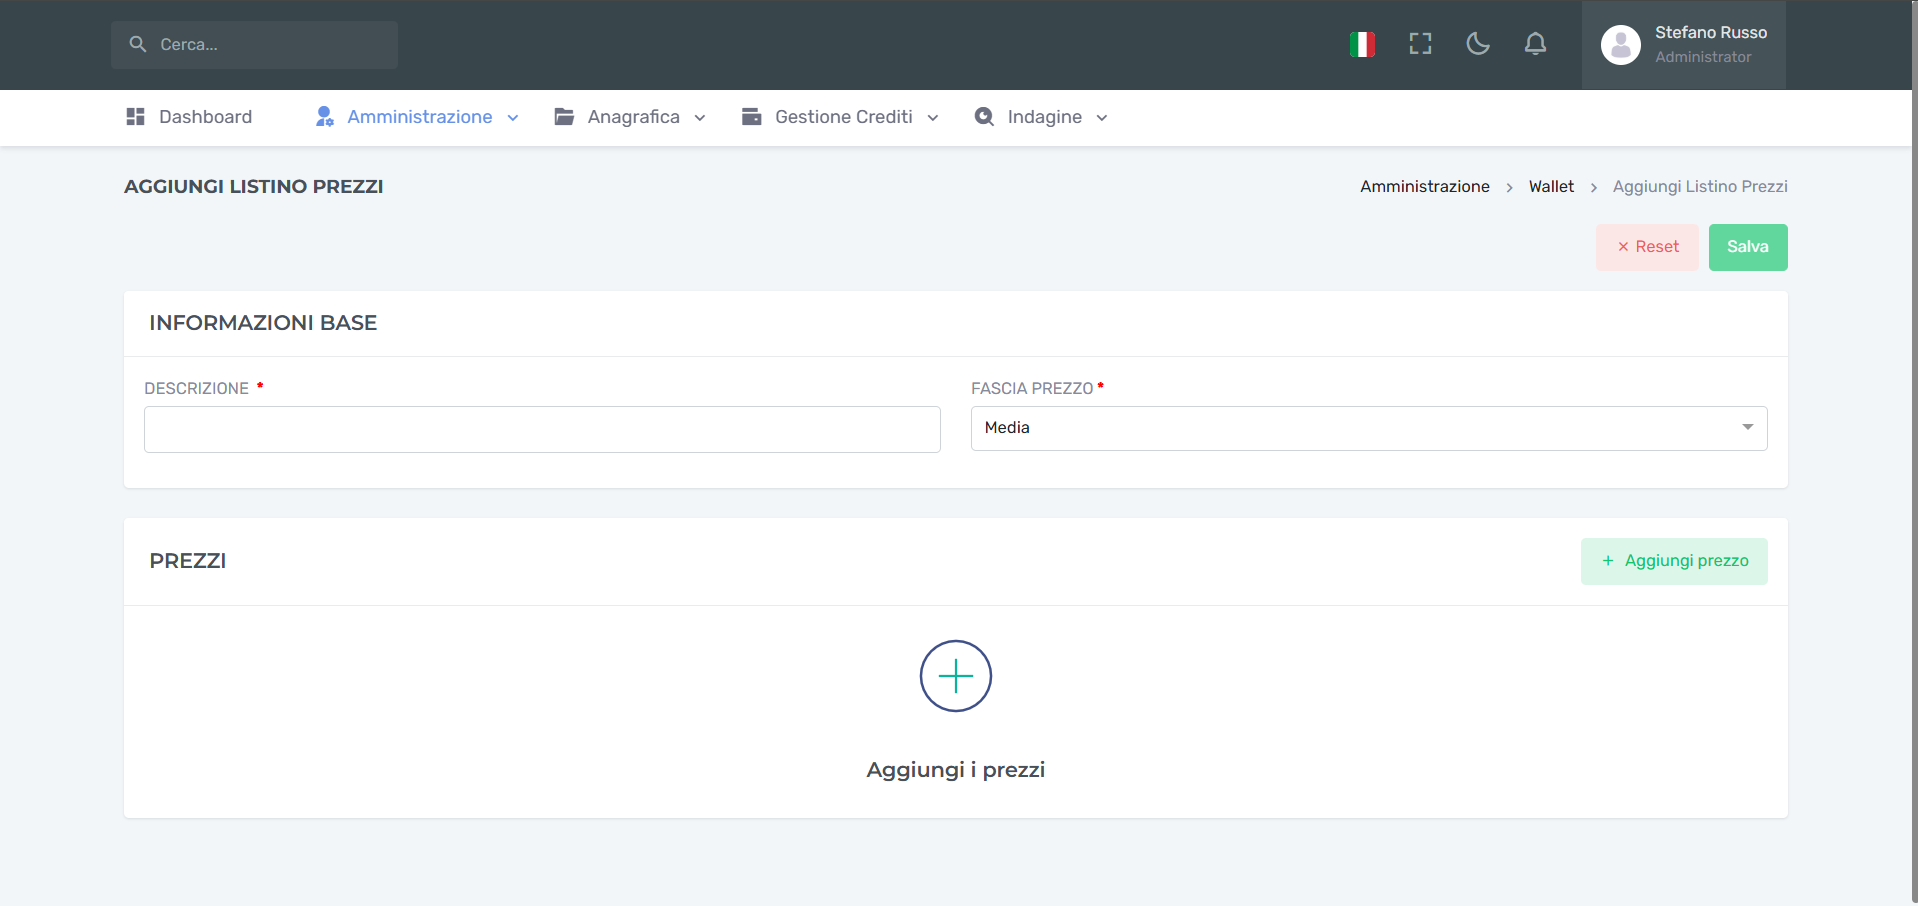
\includegraphics[width=13cm]{images/gestione-listini/screen/add-listino.png}
  \caption{Pagina di creazione di un Listino Prezzi.}
  \label{createlistinoform}
\end{figure}

Per aggiungere un prezzo \`e possibile cliccare sul relativo bottone, che aprir\`a la schermata in \textbf{Figura \ref{addpricemodal}}:
\begin{figure}[H]
  \centering
  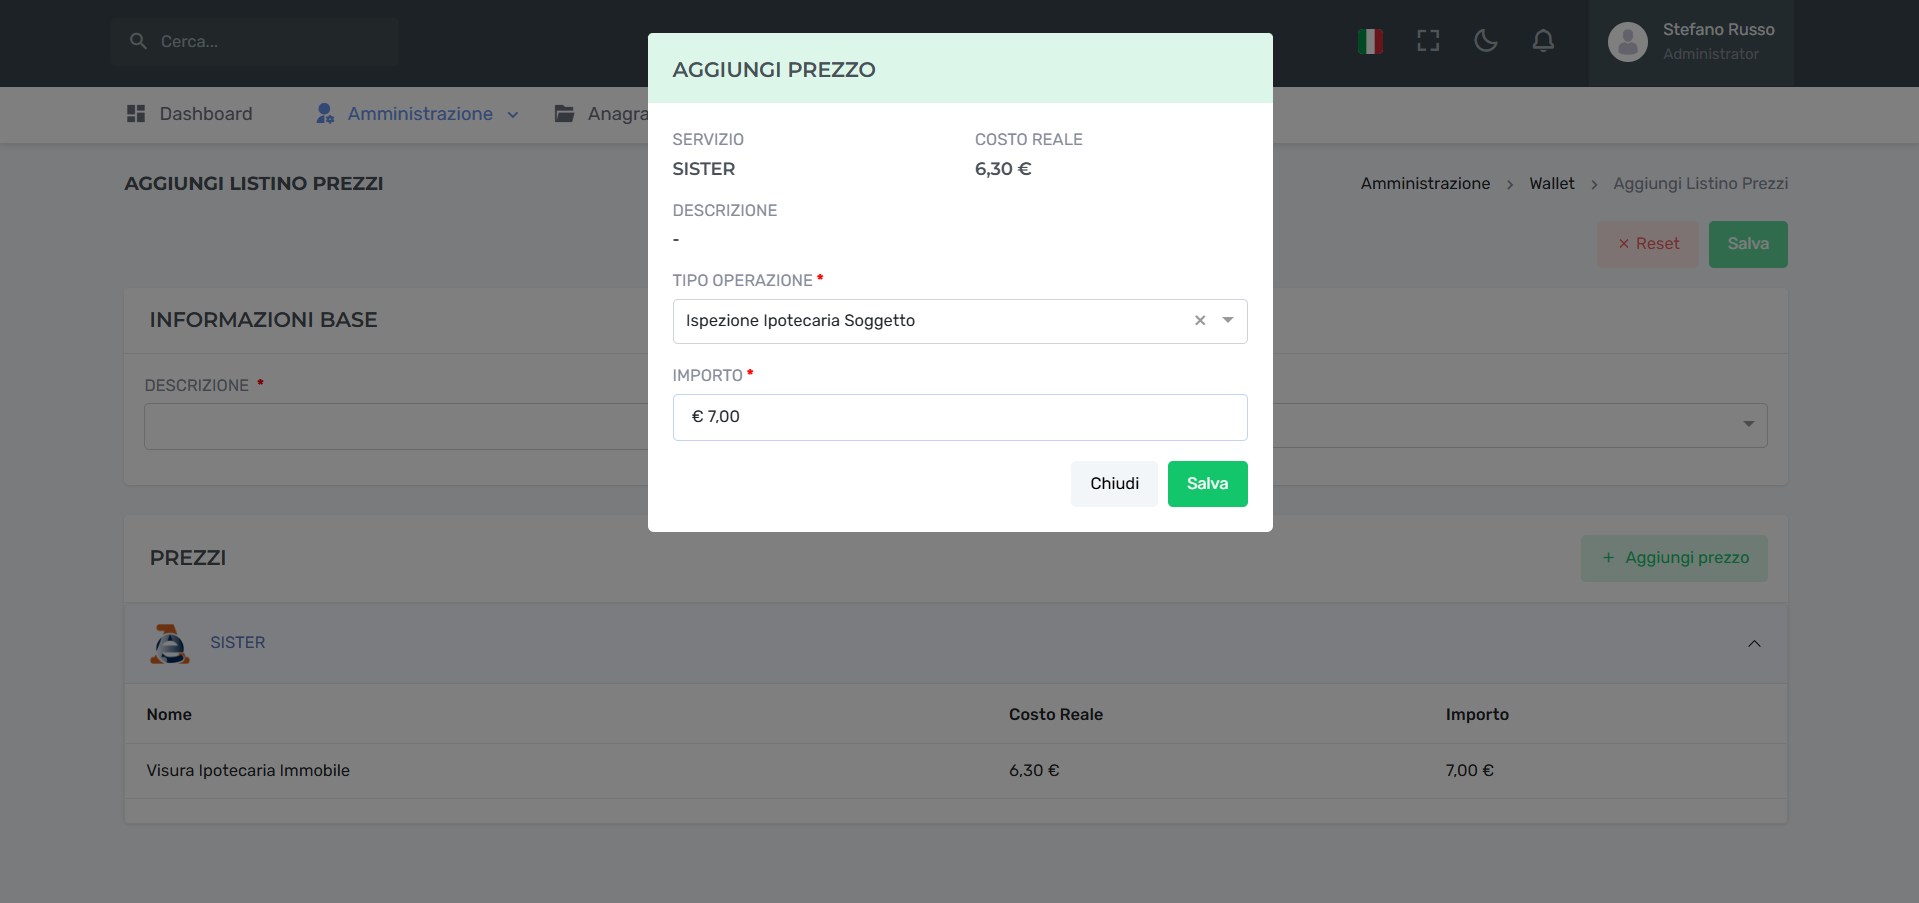
\includegraphics[width=13cm]{images/gestione-listini/screen/add-prezzo-modal.png}
  \caption{Modale per inserire un prezzo.}
  \label{addpricemodal}
\end{figure}

Dopo aver compilato i campi obbligatori del form e aver inserito un prezzo per tutte le operazioni, viene sbloccato il
tasto Salva, che invia una richiesta a questo endpoint del Credit Manager:

\subsubsection{PUT - /listino}
\begin{lstlisting}[language=Java, breaklines=true]
@PutMapping("listino")
//Controllo dei permessi generalizzato da un'annotazione.
@RfguiAuthorization(permissionId = CreditManagerConstants.WALLET_LISTINO_PREZZI_MENU_PERMISSION, writePerm = true)
public ResponseEntity<GenericResponse> createListino(HttpServletRequest req, @RequestBody CreateListinoForm form) {
  GenericResponse response = new GenericResponse();
  HttpStatus status = HttpStatus.OK;
  //Controlla che siano presenti tutti i campi obbligatori
  if (CreateListinoForm.validate(form)) {
    List<TipoOperazione> tipoOperazioneList = tipoOperazioneService.findAllExceptSentinel();
    //Controlla se ci sono tutte le operazioni. In caso negativo lancia errore, annullando la transaction
    if (!new HashSet<>(form.getPrezziListino().stream().map(PrezzoListinoForm::getTipoOperazioneId).toList()).containsAll(
            tipoOperazioneList.stream().map(TipoOperazione::getId).toList()))
        throw new InvalidFormException(HttpStatus.BAD_REQUEST, CreditManagerConstants.ERROR_INVALID_FORM);
    //Crea il listino
    Listino listino = listinoService.addListino(form.getDescrizione(), form.getFasciaPrezzo());
    //Crea un nuovo Prezzo Listino per ogni importo
    form.getPrezziListino().forEach(prezzoListino -> {
        prezzoListinoService.saveImportoForListino(prezzoListino.getTipoOperazioneId(), listino, Money.of(prezzoListino.getImporto(), "EUR"));
    });
    //Utilizza MapStruct per convertire l'entità
    response.setEntity(listinoMapper.toDTO(listino));
  } else {
    throw new InvalidFormException(HttpStatus.BAD_REQUEST, CreditManagerConstants.ERROR_INVALID_FORM);
  }
  //Se tutto è andato a buon fine, risponde al frontend col nuovo listino.
  //Termina inoltre la transaction, salvando sul database i nuovi dati.
  return ResponseEntity.status(status).body(response);
}
\end{lstlisting}
\subsubsection{Body della richiesta}
L'endpoint accetta come body oggetti definiti dalla seguente classe:

\begin{lstlisting}[language=Java, breaklines=true]
@Getter
@Setter
public class CreateListinoForm {
  private String descrizione;
  private FasciaPrezzoEnum fasciaPrezzo;
  private List<PrezzoListinoForm> prezziListino;

  public static boolean validate(CreateListinoForm form) {
    return form.getFasciaPrezzo() != null && form.getPrezziListino() != null;
  }
}
\end{lstlisting}

Come si può vedere dagli snippet di codice, anche il backend effettua un controllo per la presenza di un importo per ogni tipo operazione, garantendo che il vincolo esterno rimasto
dal passo di traduzione (\textbf{\ref{tuttiimportitraduzione}}) venga rispettato.

\section{RabbitMQ}
All'interno dell'architettura event-driven di Sentinel, il Credit Manager ha il ruolo di consumer.
Sono presenti tre Topic Exchange:
\begin{itemize}
  \item \textbf{work-exchange} - L'exchange dove vengono inviati i messaggi normalmente.
  \item \textbf{retry-exchange} - L'exchange dove vengono inviati i messaggi che hanno superato il numero massimo di retry nel work-exchange.
    Su questi messaggi viene applicato un exponential backoff, e se superano il numero massimo di retry vengono inviati nell'error-exchange. I messaggi in questo
    exchange hanno un TTL di 12000 (12 secondi).
  \item \textbf{error-exchange} - L'exchange dove vengono inviati i messaggi che hanno restituito un errore irrecuperabile o che hanno superato il numero massimo di retry.
\end{itemize}

Il Credit Manager sta in ascolto sulla coda con topic ``\#.event.payment.\#'' del work-exchange, e riceve messaggi con il seguente formato:
\begin{lstlisting}[language=Java]
public class PaymentMessage {
  private UUID idempotencyKey;
  private PaymentOperationType operationType;
  private Money costFeedback;
  private long workflowId;
}
\end{lstlisting}
Di seguito la spiegazione della funzione di ogni campo:
\begin{itemize}
  \item \textbf{idempotencyKey} - UUID che verr\`a utilizzato come chiave primaria del nuovo movimento. Permette di evitare l'inserimento
    di operazioni duplicate.
  \item \textbf{paymentOperationType} - Contiene il Tipo Operazione, equivalente a quello salvato nel database. Viene utilizzato per recuperare il costo da addebitare
    al tenant dal listino prezzi associato.
  \item \textbf{costFeedback} - \`E il costo effetivo affrontato durante l'interrogazione alla banca dati esterna. Viene registrato in caso sia differente dal costo reale associato al TipoOperazione.
  \item \textbf{workflowId} - \`E l'id del workflow, e viene utilizzato da alcuni endpoint per restituire statistiche come il totale speso in un determinato workflow.
\end{itemize}
Quando il Credit Manager riceve un messaggio sulla sua coda, registra il movimento nella tabella Movimento del database.

\section{Stripe}
Per la gestione dei pagamenti \`e stato deciso di utilizzare il Checkout di Stripe con pagina self-hosted, in modo da integrarla all'interno dell'applicativo. Un pagamento segue un flusso ben preciso:
\begin{figure}[H]
  \centering
  \hspace*{-0.55in}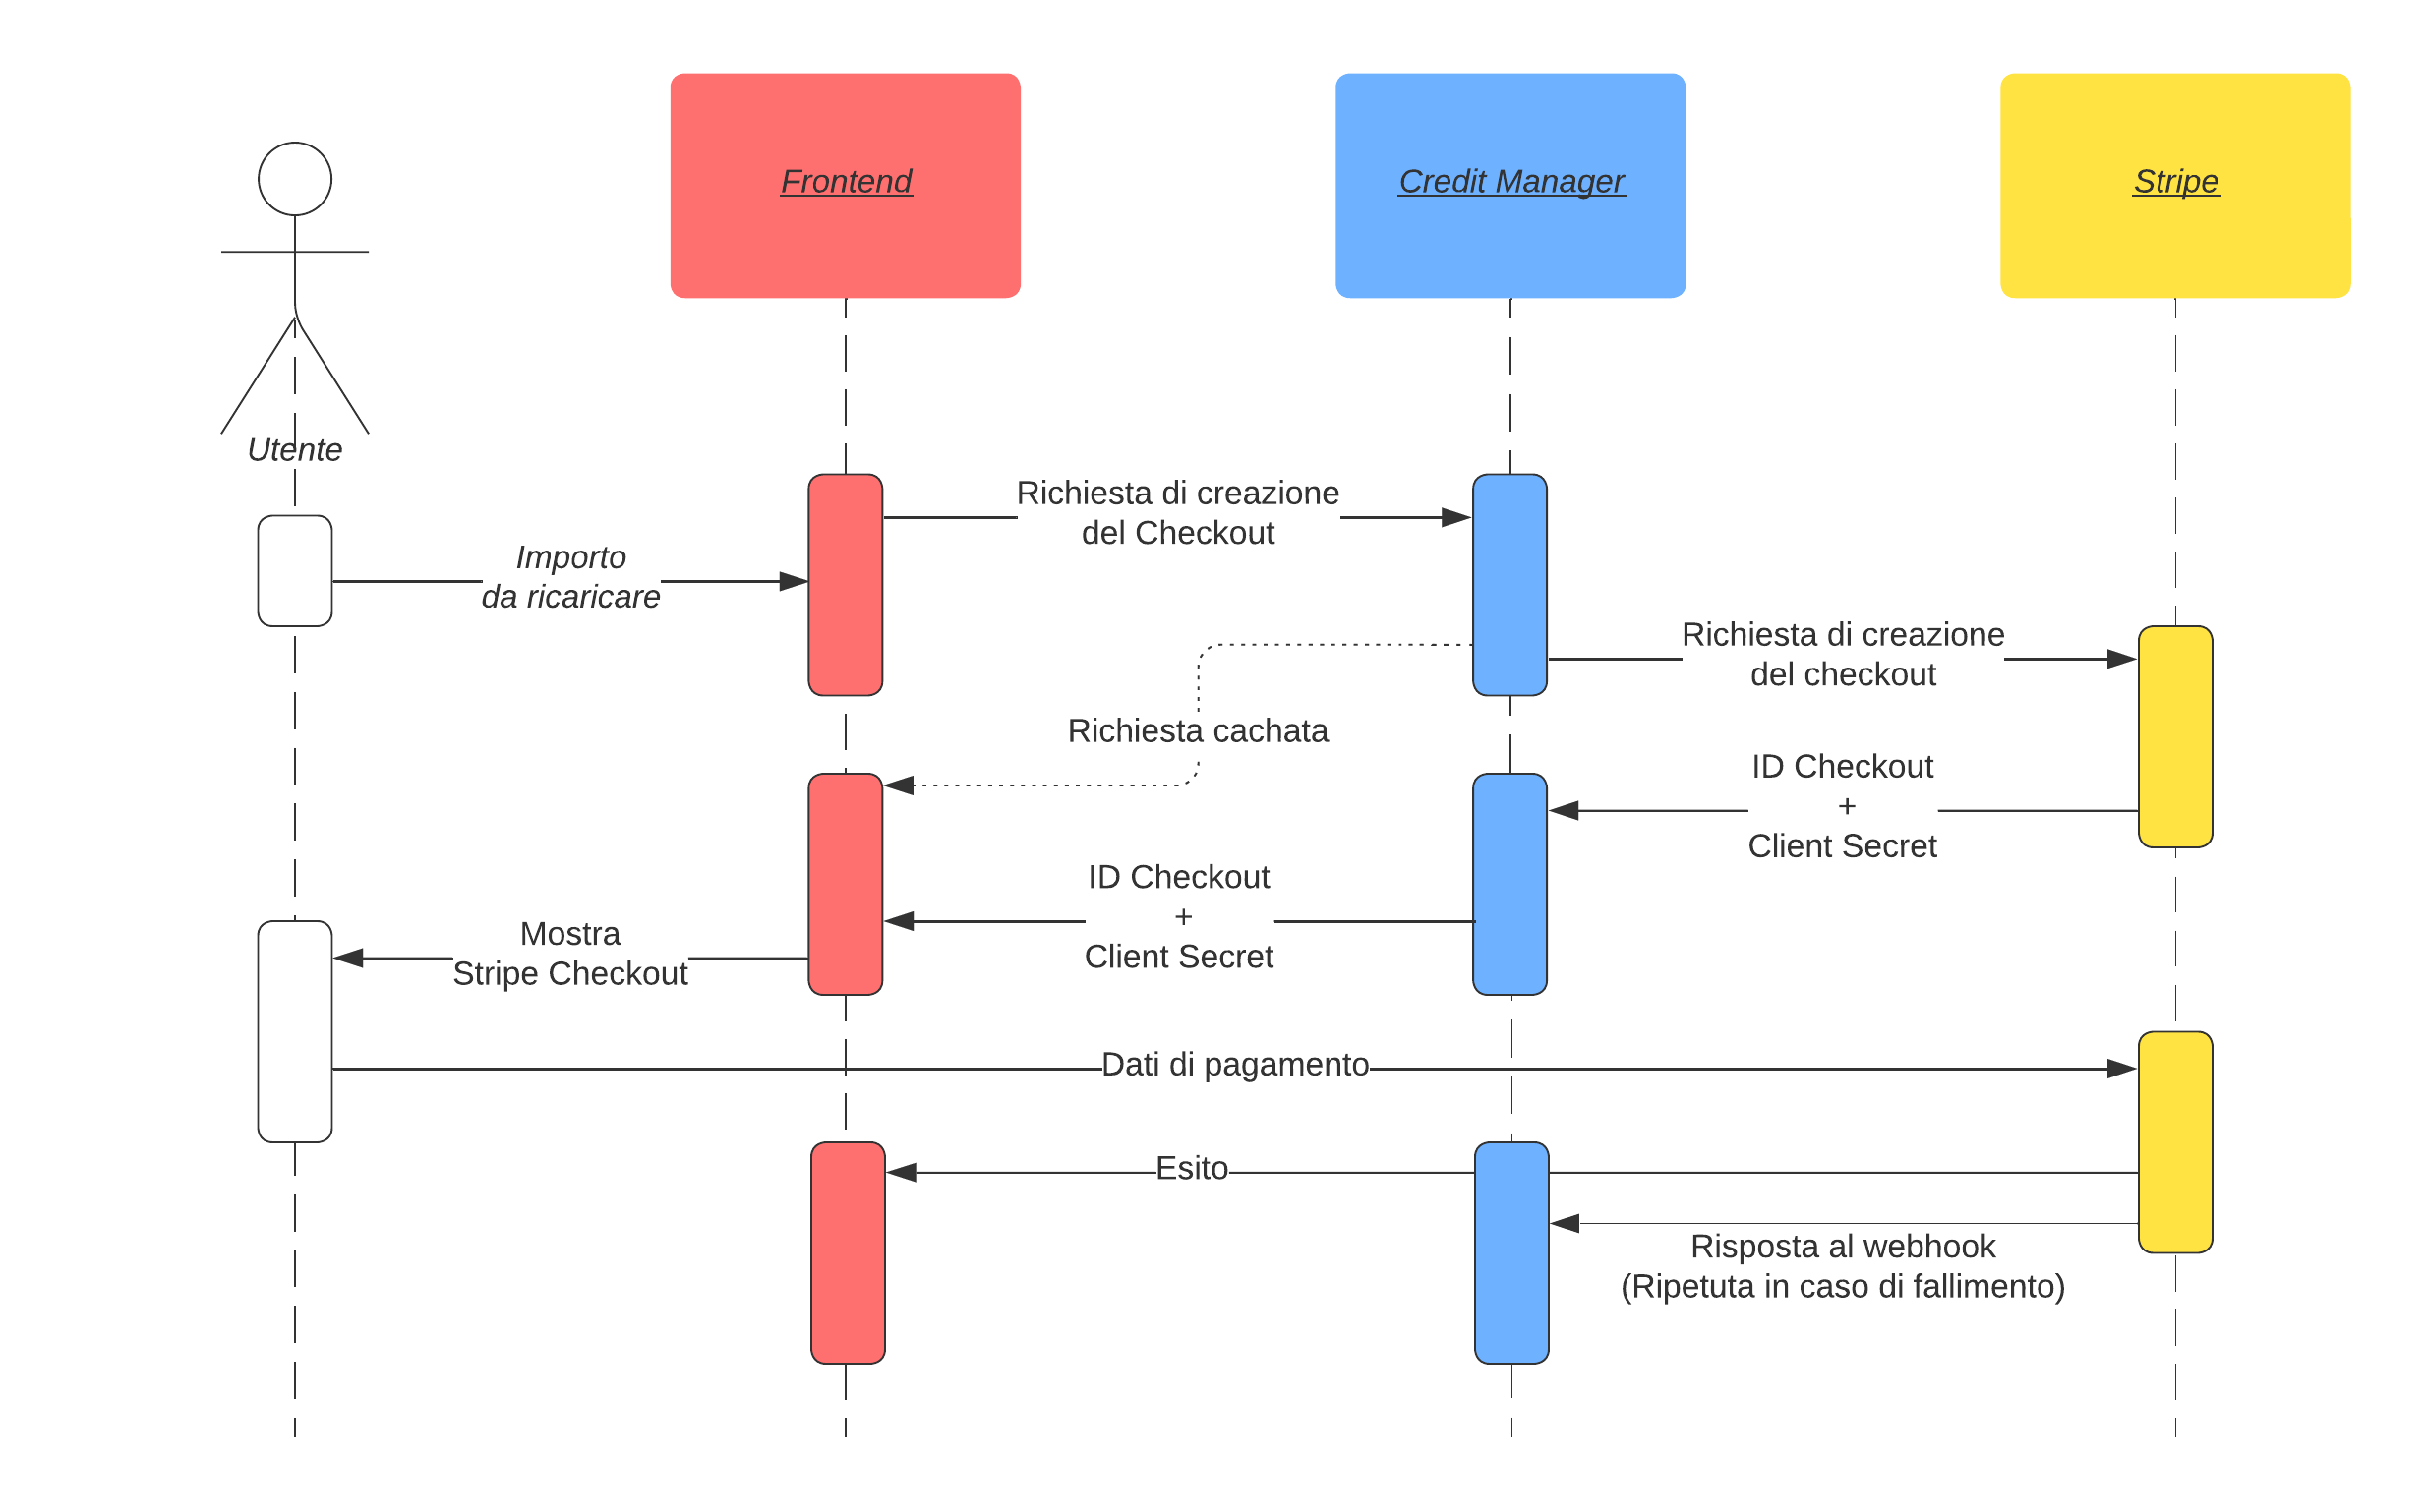
\includegraphics[width=16cm]{images/stripe-pagamento-diagramma.png}
  \caption{Diagramma di sequenza di un pagamento con Stripe}
  \label{stripepayment}
\end{figure}
\begin{enumerate}
  \item L'utente inserisce un importo maggiore di 5 euro da ricaricare e conferma.
  \item Il frontend invia l'importo con una chiave di idempotenza generata tramite UUID.
  \item Il backend verifica che la richiesta non sia gi\`a stata eseguita confrontandolo con la cache salvata su Redis, e nel caso invia al frontend la risposta precedente. In caso negativo invia a Stripe una richiesta di
    creazione del checkout con la stessa chiave di idempotenza inviata dal frontend.
  \item Stripe risponde al backend con l'id del Checkout e un Client Secret necessario per la creazione della pagina di pagamento.
  \item Il backend risponde al frontend con le informazioni inviate da Stripe.
  \item Il frontend mostra il Checkout all'utente, utilizzando i dati inviati da Stripe.
  \item L'utente inserisce i dati di pagamento e li invia attraverso l'elemento hostato da Stripe.
  \item Stripe invia l'esito sia al backend che al frontend. Nel caso del backend, l'esito viene inviato a un webhook che si occupa di registrare correttamente l'avvenuto
    pagamento. In caso il backend non restituisca il codice HTTP 200 OK, Stripe riprover\`a fino a tre giorni seguendo una strategia di Exponential Backoff.
\end{enumerate}

Il webhook ha il compito di verificare che i messaggi siano realmente provenienti da Stripe, confrontando la signature ricevuta nell'header ``Stripe-Signature'' con la
chiave ricevuta durante la configurazione del webhook.

\section{SignalStore di NgRx}
Nel corso del tirocinio \`e stata presa la decisione di ricostruire il frontend a partire da una base diversa, utilizzando l'ultima versione di Angular (Angular 17).
A tale scopo \`e stato deciso di rivedere il pattern di comunicazione tra componenti, sostituendo \textbf{NgRx} con il \textbf{SignalStore} di NgRx.
Il primo \`e un progetto che porta il pattern Redux su Angular, mentre il secondo \`e una soluzione basata interamente sui Signal, feature di Angular uscita dalla
Developer Preview proprio con la versione 17.

\`E stato quindi necessario implementare una soluzione flessibile che utilizzi al meglio il SignalStore, utilizzando quelle che vengono chiamate \textbf{feature}.
Viene fatto uso di Generics, Mapped Types, Function Overloading, e viene in generale sfruttata la capacit\`a di inferenza sui tipi di TypeScript.

Le feature implementate offrono la possibilit\`a di effettuare operazioni \textbf{CRUD} (Create, Read, Update, Delete), rimuovendo la necessit\`a di scrivere molto boilerplate e offrendo
funzionalit\`a aggiuntive ed estendibili.
Ne sono state implementate tre:
\begin{itemize}
  \item \textbf{withItem}: Si occupa di effettuare operazioni CRUD su un singolo oggetto appartenente a una collezione.
  \item \textbf{withList}: Si occupa di effettuare operazioni CRUD su una collezione.
  \item \textbf{withGrid}: Si occupa di gestire lo stato necessario per un componente generico che mostra una Tabella. Permette inoltre di effettuare operazioni CRUD sulle righe
    della tabella stessa.
\end{itemize}

Prenderemo in esame withGrid, la pi\`u complessa.
\\
\begin{figure}[H]
  \centering
  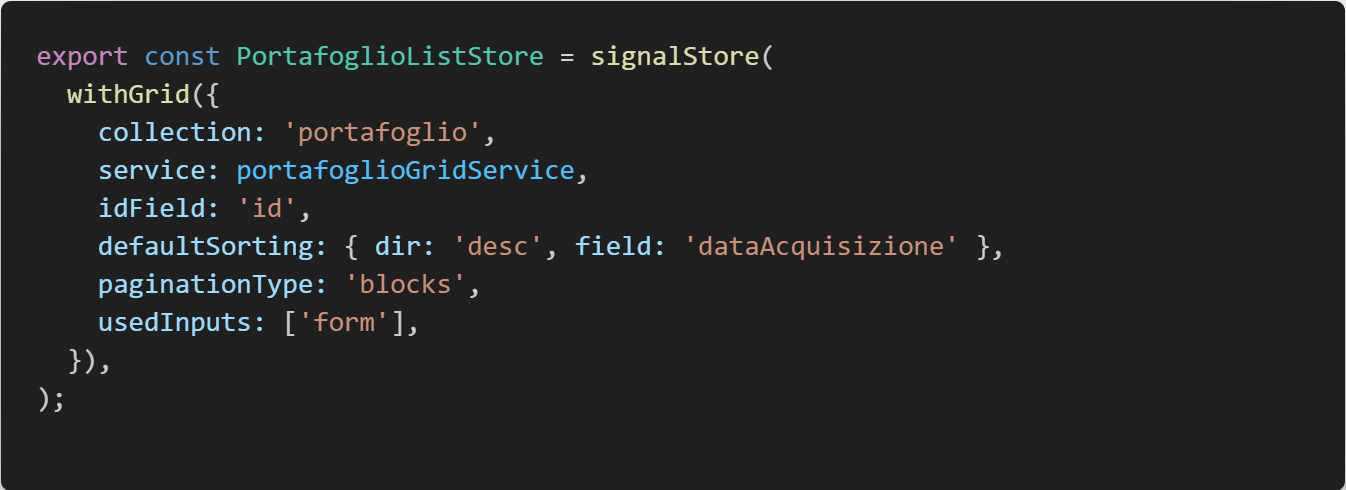
\includegraphics[width=12cm]{images/code-store.png}
  \caption{Codice per creare uno Store con withGrid}
\end{figure}

Questo \`e il codice richiesto per creare uno Store che include withGrid. La feature prende in input diversi parametri:
\begin{itemize}
  \item \textbf{collection} - La stringa su cui verranno basati i nomi delle funzioni CRUD e dello stato.
  \item \textbf{service} - Oggetto che contiene i metodi che comunicano con il backend. Restituiscono
    l'\textbf{Observable}\footnote{Un Observable \`e la base della reattivit\`a fornita da RxJs: \`e una sorgente di dati che vengono emessi nel tempo.
      Il flusso pu\`o essere manipolato appendendo degli operatori che modificano il dato ad ogni passo. I pi\`u comuni sono map e filter.
    Angular li utilizza per le chiamate HTTP, e in questo caso emettono un valore una sola volta per subscription.}
    a cui lo store si sottoscriver\`a
    per effettuare la chiamata. \`E stato disposto un tipo generico che prende in input i tipi per definire i parametri necessari per le chiamate, tra cui il tipo
    dell'oggetto che lo Store deve gestire, o i routeParams che deve utilizzare per generare l'URL. Questo tipo generico consente a IDE moderni come Visual Studio Code di
    generare tutte le funzioni che poi verranno chiamate dalla feature.
  \item \textbf{paginationType} - Il tipo di paginazione utilizzato. Ha tre possibili valori: \textbf{none}, \textbf{blocks}, \textbf{pages}. Questo perch\'e lo store
    gestisce anche la paginazione per il componente generico, e si deve comportare in maniera diversa a seconda del tipo. Per blocks, la paginazione e il sorting
    vengono gestiti dal backend, che prende in input anche la dimensione e il numero del blocco. Nel caso di pages invece, la paginazione \`e interamente gestita
    dalla feature e dal componente generico. Se il valore di paginationType \`e none viene disabilitata la paginazione.
  \item \textbf{idField} - Nome del campo ID dell'oggetto che la grid sta trattando. Il valore di questo campo deve essere necessariamente univoco negli oggetti inseriti,
    in quanto necessario per il corretto funzionamento della feature e del componente generico (per esempio, viene utilizzato nel track del @for di Angular).
  \item \textbf{defaultSorting} - Valore iniziale del campo per cui vengono ordinati gli oggetti all'interno della grid. Nella paginazione a blocchi questo valore viene inviato
    anche al backend, altrimenti viene utilizzato localmente.
  \item \textbf{usedInputs} - Valore utilizzato internamente dalla feature per abilitare o disabilitare determinati input. Il suo valore viene forzato attraverso il typing system
    di TypeScript utilizzando il tipo di Service.
\end{itemize}

La feature mette a disposizione diverse funzioni e valori: tutte le tipiche funzioni CRUD, una funzione per effettuare il reload della grid con gli ultimi input passati,
e lo stato dell'ultima chiamata effettuata (Loading, Loaded, Error, o Init se non \`e stata effettuata nessuna chiamata dalla creazione dello store).

Prendiamo ora come esempio il codice necessario per definire un service per withGrid:
\begin{figure}[H]
  \centering
  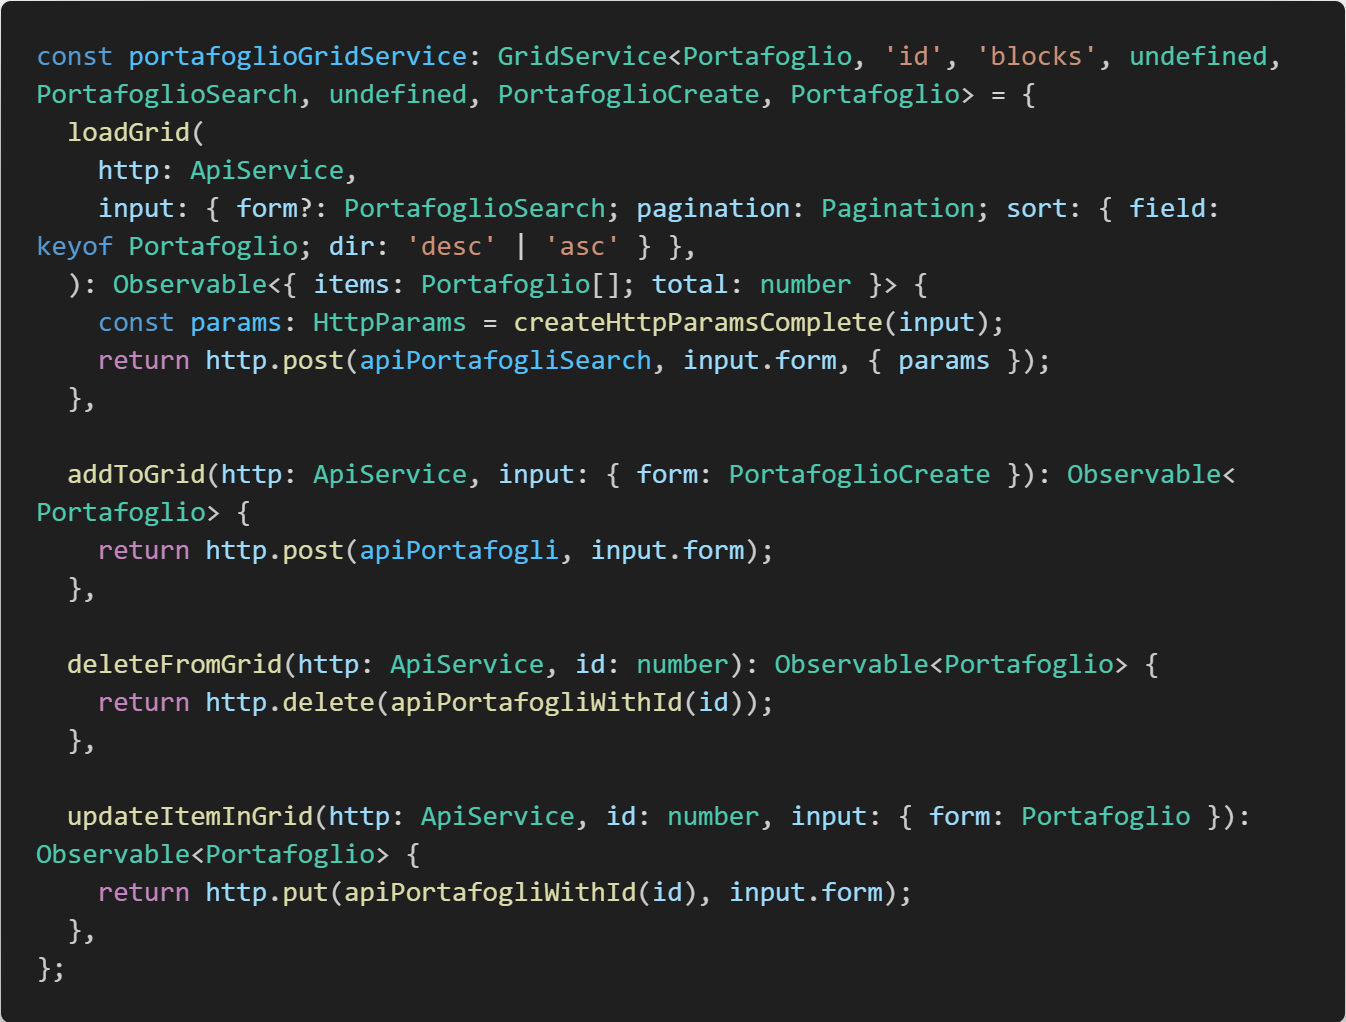
\includegraphics[width=12cm]{images/code-service.png}
  \caption{Codice del servizio con le chiamate al backend}
\end{figure}
Come mostrato dal codice in figura, \`e necessario passare diverse informazioni al tipo GridService per permettere a TypeScript di effettuare tutte le inferenze sui tipi:
\begin{itemize}
  \item \textbf{Tipo dell'Entit\`a} - Tipo dell'oggetto popolato nello stato. Viene utilizzato da TypeScript per le inferenze all'interno del Signalstore e
    per l'autocompletamento delle funzioni del Service stesso.
  \item \textbf{Nome del campo ID} - Uguale a quello specificato sopra. L'uguaglianza viene forzata dal typing system.
  \item \textbf{Tipo di paginazione} - Stesso tipo di paginazione specificato sopra. L'uguaglianza viene forzata dal typing system.
  \item \textbf{RouteParams} - Campo per specificare RouteParams obbligatori utilizzati per la costruzione degli URL nelle funzioni.
  \item \textbf{Form} - Dato che tipicamente questa feature viene utilizzata per tabelle con filtri, \`e necessario includere un body con i parametri per effettuare la ricerca.
  \item \textbf{QueryParams} - Campo per i QueryParams opzionali utilizzati nelle funzioni.
  \item \textbf{FormCreate} - Form utilizzato dalla funzione addToGrid.
  \item \textbf{FormUpdate} - Form utilizzato dalla funzione updateItemInGrid.
\end{itemize}
